% ═══════════════════════════════════════════════════════════════════════════
%  DDF — préambule commun aux sept articles.  % ═══════════════════════════════════════════════════════════════════════════
%  DDF — préambule commun aux sept articles.  % ═══════════════════════════════════════════════════════════════════════════
%  DDF — préambule commun aux sept articles.  \input{ddf-common} en tête.
%  Définit : la mise en page, les macros, le bloc de série, la déclaration
%  d'usage d'outils, et le bloc de traçabilité.
% ═══════════════════════════════════════════════════════════════════════════
\documentclass[11pt,a4paper]{article}
\usepackage[margin=2.3cm]{geometry}
\usepackage{amsmath,amssymb,booktabs,hyperref,graphicx,xcolor}
\usepackage[expansion=false]{microtype}
\hypersetup{colorlinks=true,linkcolor=blue!45!black,citecolor=blue!45!black,urlcolor=blue!45!black}

% ---------- macros physiques ----------
\newcommand{\MPl}{M_{\rm Pl}}\newcommand{\Mred}{\bar M_{\rm Pl}}
\newcommand{\Mfive}{M_5}\newcommand{\MS}{M_S}\newcommand{\V}{\mathcal V}
\newcommand{\Neff}{N_{\rm eff}}\newcommand{\cb}{c_b}\newcommand{\ab}{\alpha_b}

% ---------- étiquettes épistémiques ----------
\newcommand{\Derived}{\textit{[Derived]}}
\newcommand{\Input}{\textit{[Input, natural]}}
\newcommand{\Posited}{\textit{[Posited]}}
\newcommand{\Candidate}{\textit{[Candidate]}}
\newcommand{\Open}{\textit{[Open, declared]}}
\newcommand{\Verified}{\textit{[Verified]}}

% ---------- bloc de série : \seriesdate{III}{The medium} ----------
\newcommand{\seriesdate}[2]{%
 \date{\small \textit{Cosmic Shadow Geometry} \\ \small Article #1 of VII
 \,\textperiodcentered\, #2 \,\textperiodcentered\, \today}}

% ---------- déclaration d'outils, identique dans les sept ----------
\newcommand{\toolsstatement}{%
\section*{Declaration on computational tools}
\addcontentsline{toc}{section}{Declaration on computational tools}
\small
This work was carried out by the author alone, without institutional affiliation.
\textbf{Large language models were used as computational and analytical assistants
throughout}: to write and debug the numerical scripts, to run the scans and
minimisations, to produce the figures, to check algebra and dimensional
consistency, to search and summarise the literature, and to audit drafts for
internal contradictions. Several distinct systems were used and cross-checked
against one another; no single system's output was accepted without an
independent numerical or analytical verification.

\textbf{The author is solely responsible for the physical hypotheses, the
interpretation of every result, the epistemic labels attached to each claim, and
the decision of what to publish and what to withdraw.} All quantitative
statements in this paper are reproduced by the scripts listed in the
traceability section; a reader who runs them obtains the numbers printed here
without needing any language model. Where an earlier draft contained an error
introduced by an unverified computation, it is recorded as a withdrawal rather
than silently removed.
\normalsize}

% ---------- bloc de traçabilité : \traceability{V}{...} ----------
\newcommand{\traceability}[2]{%
\section*{Data availability, traceability and reproducibility}
\addcontentsline{toc}{section}{Traceability}
\small
Every number, table and figure in this paper is regenerated by the scripts of
this article's folder. The complete repository ---sources, scripts, proof files,
figures and compiled documents for all seven articles--- is at
\url{https://github.com/HBoufourou}.

\textbf{Folder \texttt{article-#1/} contains:}
\begin{itemize}\itemsep2pt
\item \texttt{tex/} --- the \LaTeX\ source and the shared preamble \texttt{ddf-common.tex};
\item \texttt{scripts/} --- every computation, each runnable standalone with
      \texttt{python3 <name>.py} and printing its own verification verdict;
\item \texttt{proofs/} --- the JSON files carrying the certified values.
      \textbf{Any number absent from \texttt{proofs/} is not certified};
\item \texttt{data/} --- the CSV tables underlying the figures;
\item \texttt{figures/} --- the PNG files, regenerated by \texttt{scripts/figures.py};
\item \texttt{pdf/} --- the compiled article;
\item \texttt{VERIFICATION.txt} --- the output of the verification suite.
\end{itemize}
#2
\normalsize}
 en tête.
%  Définit : la mise en page, les macros, le bloc de série, la déclaration
%  d'usage d'outils, et le bloc de traçabilité.
% ═══════════════════════════════════════════════════════════════════════════
\documentclass[11pt,a4paper]{article}
\usepackage[margin=2.3cm]{geometry}
\usepackage{amsmath,amssymb,booktabs,hyperref,graphicx,xcolor}
\usepackage[expansion=false]{microtype}
\hypersetup{colorlinks=true,linkcolor=blue!45!black,citecolor=blue!45!black,urlcolor=blue!45!black}

% ---------- macros physiques ----------
\newcommand{\MPl}{M_{\rm Pl}}\newcommand{\Mred}{\bar M_{\rm Pl}}
\newcommand{\Mfive}{M_5}\newcommand{\MS}{M_S}\newcommand{\V}{\mathcal V}
\newcommand{\Neff}{N_{\rm eff}}\newcommand{\cb}{c_b}\newcommand{\ab}{\alpha_b}

% ---------- étiquettes épistémiques ----------
\newcommand{\Derived}{\textit{[Derived]}}
\newcommand{\Input}{\textit{[Input, natural]}}
\newcommand{\Posited}{\textit{[Posited]}}
\newcommand{\Candidate}{\textit{[Candidate]}}
\newcommand{\Open}{\textit{[Open, declared]}}
\newcommand{\Verified}{\textit{[Verified]}}

% ---------- bloc de série : \seriesdate{III}{The medium} ----------
\newcommand{\seriesdate}[2]{%
 \date{\small \textit{Cosmic Shadow Geometry} \\ \small Article #1 of VII
 \,\textperiodcentered\, #2 \,\textperiodcentered\, \today}}

% ---------- déclaration d'outils, identique dans les sept ----------
\newcommand{\toolsstatement}{%
\section*{Declaration on computational tools}
\addcontentsline{toc}{section}{Declaration on computational tools}
\small
This work was carried out by the author alone, without institutional affiliation.
\textbf{Large language models were used as computational and analytical assistants
throughout}: to write and debug the numerical scripts, to run the scans and
minimisations, to produce the figures, to check algebra and dimensional
consistency, to search and summarise the literature, and to audit drafts for
internal contradictions. Several distinct systems were used and cross-checked
against one another; no single system's output was accepted without an
independent numerical or analytical verification.

\textbf{The author is solely responsible for the physical hypotheses, the
interpretation of every result, the epistemic labels attached to each claim, and
the decision of what to publish and what to withdraw.} All quantitative
statements in this paper are reproduced by the scripts listed in the
traceability section; a reader who runs them obtains the numbers printed here
without needing any language model. Where an earlier draft contained an error
introduced by an unverified computation, it is recorded as a withdrawal rather
than silently removed.
\normalsize}

% ---------- bloc de traçabilité : \traceability{V}{...} ----------
\newcommand{\traceability}[2]{%
\section*{Data availability, traceability and reproducibility}
\addcontentsline{toc}{section}{Traceability}
\small
Every number, table and figure in this paper is regenerated by the scripts of
this article's folder. The complete repository ---sources, scripts, proof files,
figures and compiled documents for all seven articles--- is at
\url{https://github.com/HBoufourou}.

\textbf{Folder \texttt{article-#1/} contains:}
\begin{itemize}\itemsep2pt
\item \texttt{tex/} --- the \LaTeX\ source and the shared preamble \texttt{ddf-common.tex};
\item \texttt{scripts/} --- every computation, each runnable standalone with
      \texttt{python3 <name>.py} and printing its own verification verdict;
\item \texttt{proofs/} --- the JSON files carrying the certified values.
      \textbf{Any number absent from \texttt{proofs/} is not certified};
\item \texttt{data/} --- the CSV tables underlying the figures;
\item \texttt{figures/} --- the PNG files, regenerated by \texttt{scripts/figures.py};
\item \texttt{pdf/} --- the compiled article;
\item \texttt{VERIFICATION.txt} --- the output of the verification suite.
\end{itemize}
#2
\normalsize}
 en tête.
%  Définit : la mise en page, les macros, le bloc de série, la déclaration
%  d'usage d'outils, et le bloc de traçabilité.
% ═══════════════════════════════════════════════════════════════════════════
\documentclass[11pt,a4paper]{article}
\usepackage[margin=2.3cm]{geometry}
\usepackage{amsmath,amssymb,booktabs,hyperref,graphicx,xcolor}
\usepackage[expansion=false]{microtype}
\hypersetup{colorlinks=true,linkcolor=blue!45!black,citecolor=blue!45!black,urlcolor=blue!45!black}

% ---------- macros physiques ----------
\newcommand{\MPl}{M_{\rm Pl}}\newcommand{\Mred}{\bar M_{\rm Pl}}
\newcommand{\Mfive}{M_5}\newcommand{\MS}{M_S}\newcommand{\V}{\mathcal V}
\newcommand{\Neff}{N_{\rm eff}}\newcommand{\cb}{c_b}\newcommand{\ab}{\alpha_b}

% ---------- étiquettes épistémiques ----------
\newcommand{\Derived}{\textit{[Derived]}}
\newcommand{\Input}{\textit{[Input, natural]}}
\newcommand{\Posited}{\textit{[Posited]}}
\newcommand{\Candidate}{\textit{[Candidate]}}
\newcommand{\Open}{\textit{[Open, declared]}}
\newcommand{\Verified}{\textit{[Verified]}}

% ---------- bloc de série : \seriesdate{III}{The medium} ----------
\newcommand{\seriesdate}[2]{%
 \date{\small \textit{Cosmic Shadow Geometry} \\ \small Article #1 of VII
 \,\textperiodcentered\, #2 \,\textperiodcentered\, \today}}

% ---------- déclaration d'outils, identique dans les sept ----------
\newcommand{\toolsstatement}{%
\section*{Declaration on computational tools}
\addcontentsline{toc}{section}{Declaration on computational tools}
\small
This work was carried out by the author alone, without institutional affiliation.
\textbf{Large language models were used as computational and analytical assistants
throughout}: to write and debug the numerical scripts, to run the scans and
minimisations, to produce the figures, to check algebra and dimensional
consistency, to search and summarise the literature, and to audit drafts for
internal contradictions. Several distinct systems were used and cross-checked
against one another; no single system's output was accepted without an
independent numerical or analytical verification.

\textbf{The author is solely responsible for the physical hypotheses, the
interpretation of every result, the epistemic labels attached to each claim, and
the decision of what to publish and what to withdraw.} All quantitative
statements in this paper are reproduced by the scripts listed in the
traceability section; a reader who runs them obtains the numbers printed here
without needing any language model. Where an earlier draft contained an error
introduced by an unverified computation, it is recorded as a withdrawal rather
than silently removed.
\normalsize}

% ---------- bloc de traçabilité : \traceability{V}{...} ----------
\newcommand{\traceability}[2]{%
\section*{Data availability, traceability and reproducibility}
\addcontentsline{toc}{section}{Traceability}
\small
Every number, table and figure in this paper is regenerated by the scripts of
this article's folder. The complete repository ---sources, scripts, proof files,
figures and compiled documents for all seven articles--- is at
\url{https://github.com/HBoufourou}.

\textbf{Folder \texttt{article-#1/} contains:}
\begin{itemize}\itemsep2pt
\item \texttt{tex/} --- the \LaTeX\ source and the shared preamble \texttt{ddf-common.tex};
\item \texttt{scripts/} --- every computation, each runnable standalone with
      \texttt{python3 <name>.py} and printing its own verification verdict;
\item \texttt{proofs/} --- the JSON files carrying the certified values.
      \textbf{Any number absent from \texttt{proofs/} is not certified};
\item \texttt{data/} --- the CSV tables underlying the figures;
\item \texttt{figures/} --- the PNG files, regenerated by \texttt{scripts/figures.py};
\item \texttt{pdf/} --- the compiled article;
\item \texttt{VERIFICATION.txt} --- the output of the verification suite.
\end{itemize}
#2
\normalsize}

\graphicspath{{figures/}{../figures/}}
\title{\textbf{The Dark Dimension Framework II:\\ The well and the tower --- the meV sector from brane sources}}
\author{Hicham Boufourou\\ \small\textit{Independent Researcher, Brussels, Belgium}\\ \small\texttt{hicham.boufourou@hotmail.com}}
\seriesdate{II}{The well and the tower}
\begin{document}\maketitle
\begin{abstract}
\noindent The dark sector of the Dark Dimension Framework is a single bulk scalar $\Phi$ confined against our wall by a potential linear in the bulk coordinate, whose bound states form a discrete tower. Earlier statements of the framework posited that linear potential; this article derives it, and in doing so closes the amplitude accounting of the whole series. Two independent brane sources produce the same linear well. The first is gravitational and comes for free: the tension of the thin core of Article I pulls on any bulk field, giving a slope $F=m_{\Phi}\kappa_{5}^{2}T/6$; reproducing the observed slope requires $T^{1/4}=9.8$~TeV, inside the one-scale wall window --- the well is, in this road, the brane's own gravity at work. The second is field-theoretic and unique at the minimal level: a $\mathbb{Z}_{2}$-even bulk scalar $\sigma$ sourced by boundary tadpoles obeys Laplace's equation in the empty bulk, so its profile is \emph{exactly} linear with zero shape parameters; parity excludes the odd assignment outright, and Gauss's law on the compact interval forces the two tadpoles to be equal and opposite. On the derived well the interleaved tower --- even branch Neumann at the sourced wall, odd branch Dirichlet --- has ratios $1:2.29:3.19:4.03$ with nothing adjusted, and the interval-to-well ratio is itself an output: $u=\pi R/\ell=4.43$, closing the triplet $(\ell,\varepsilon,u)$ on the single scale $m_{\Phi}=\varepsilon\approx1/R=24$~meV. The construction returns two dials: a nonzero source mass bends the profile into $\sinh$, and tower ratios measured at $1\%$ bound $m_{\sigma}<4.3$~meV; and the fourth ratio, the only level that feels the far wall, measures $u$ itself. The ground state's boundary weight is computed, $w_{1}=5.5$, so the covariant vertex of Article I gives the galactic amplitude $\alpha_{b}=3.3\,c_{b}$, translating the framework's requirement table into $c_{b}=0.30$--$0.61$ for the benchmark responses --- order unity, with nothing forced. The source field leaves no trace elsewhere: ordinary matter carries no $\sigma$ charge, so the tree-level fifth force vanishes and the short-range landscape of Article I is unchanged; induced channels are bounded below $10^{-100}$ of gravity. Two shadows are declared rather than hidden: the $\Lambda$ budget caps the tadpole and thereby demands a coupling $\sim2\times10^{3}$ above its natural size --- a tension of the cosmological-constant class, shown to survive both a 't Hooft analysis and TeV-scale supersymmetry --- and the same field cannot stabilise the radius, its contribution to the radion mass falling twenty-eight orders short, so the TeV core and the meV source sector are genuinely independent origins, a structure Article IV will explain rather than repair.
\end{abstract}

\section{Purpose: from posited to computed}
Article I built the stage; this article builds what lives in it. The object is the framework's single dark degree of freedom, a bulk scalar $\Phi$ of mass $m_{\Phi}$, and the structure that organises everything downstream --- the reservoir and mediator roles of Article III, the galactic response, the cosmological history --- is its discrete spectrum in a confining well linear in the bulk coordinate $y$:
\begin{equation}
V_{\rm eff}(y)=F\,y ,\qquad y\in[0,\pi R].
\end{equation}
In earlier statements of this framework the linearity of $V_{\rm eff}$ was an input. Here it is a result, obtained twice by independent roads, each bringing its own observable; and with the well derived, the boundary weight of its ground state can be computed rather than parametrised, which closes the amplitude accounting left open by Article I's vertex. The labels and rules of the series apply throughout; every number below is reproduced by the dossier scripts. This framework is a dark dimension in the sense of Montero, Vafa and Valenzuela; the name records its central structure, the shadow relation of Article~IV, under which the entire millielectronvolt sector is the gravitational shadow of one TeV scale. A fifth article, cited throughout as the \emph{companion}, examines whether this geometry admits an ultraviolet completion in Type~I$'$ string theory; it is a companion, not a foundation, and nothing in Articles~I--IV depends on it.

\section{Two roads to the same well}
\subsection{The gravitational road: the brane's own pull}
The thin core of Article I carries tension $T$, and tension gravitates. In the linearised five-dimensional metric sourced by the wall, any bulk field of mass $m_{\Phi}$ feels a potential rising linearly off the brane with slope
\begin{equation}
F_{\rm grav}=\frac{m_{\Phi}\,\kappa_{5}^{2}\,T}{6},\qquad \kappa_{5}^{2}=\Mfive^{-3},
\label{eq:gravslope}
\end{equation}
the five-dimensional analogue of a ball resting on a stretched membrane. This road is parameter-free once $T$ is given, and it can be inverted: the observed slope of the dark sector, $F=8.15\times10^{-22}~\mathrm{GeV}^{2}$ (fixed below by the tower scale), requires
\begin{equation}
T^{1/4}=9.8~\mathrm{TeV},
\end{equation}
squarely inside the one-scale wall window $m_{\chi}\sim1$--$10$~TeV of Article I, and --- a consistency Article IV will elevate to structure --- inside the same band that the framework's other TeV quantities occupy. Binding between one and four tower levels inside the interval brackets the tension at $T^{1/4}\in2$--$13$~TeV, which is where Article I's window came from. In this road, \emph{the well is the brane's own gravity}: the dark tower hangs on the wall the way the neutron's gravitational states hang on the Earth. [Derived]

\subsection{The field road: the capacitor}
The second road asks what \emph{minimal field content} produces a linear profile, and the answer is forced at every step. Let $\sigma$ be a bulk scalar with boundary sources,
\begin{equation}
S_{\rm src}=\int d^{4}x\left[\,J_{0}\,\sigma(x,0)+J_{\pi}\,\sigma(x,\pi R)\,\right],
\end{equation}
coupled to the dark field by $g\,\Phi^{2}\sigma$. Three structural statements make the construction unique at the minimal level. \emph{Parity:} the coupling must be $\mathbb{Z}_{2}$-even to exist in the orbifold action; $\Phi^{2}$ is even, so $\sigma$ must be even --- the odd assignment is excluded outright, not suppressed. \emph{Laplace:} in the empty bulk the static profile obeys $\sigma''=m_{\sigma}^{2}\sigma$; for $m_{\sigma}\to0$ this is Laplace's equation, whose solution on the covering space is $\sigma(y)=\sigma_{0}-(J_{0}/2)\,|y|$ --- even, with the fold at the boundary being the source itself --- hence \emph{exactly linear} on the physical interval, with zero shape parameters. The induced slope is
\begin{equation}
F_{\rm cap}=\tfrac{1}{2}\,g\,J_{0},
\end{equation}
the factor two being the orbifold fold. \emph{Gauss:} on a compact space a massless field's total source must vanish, $J_{0}+J_{\pi}=0$: the equal-and-opposite tadpoles of the capacitor are not chosen, they are forced (relaxing to $J_{0}+J_{\pi}=\mathcal{O}((m_{\sigma}\pi R)^{2})$ for a massive source). A scale consistency comes for free: $\sqrt{F}=29$~meV, the scale of the tower itself --- the source sector lives at the millielectronvolt scale of the dark sector, cleanly thirteen orders below the TeV core. [Derived]

\subsection{Which road carries the well}
Both roads produce the same functional form, so the physical slope is their sum, and the framework does not need to choose: the gravitational contribution is fixed by $T$ and automatically in range, while the capacitor adds a field-theoretic channel whose mass $m_{\sigma}$ becomes measurable (\S4). What matters for everything downstream is the linearity itself, now doubly derived, and the single number $F$ --- which the tower fixes. [Derived; attribution between roads: Open, and testable through the $m_{\sigma}$ dial]

\begin{figure}[t]
\centering
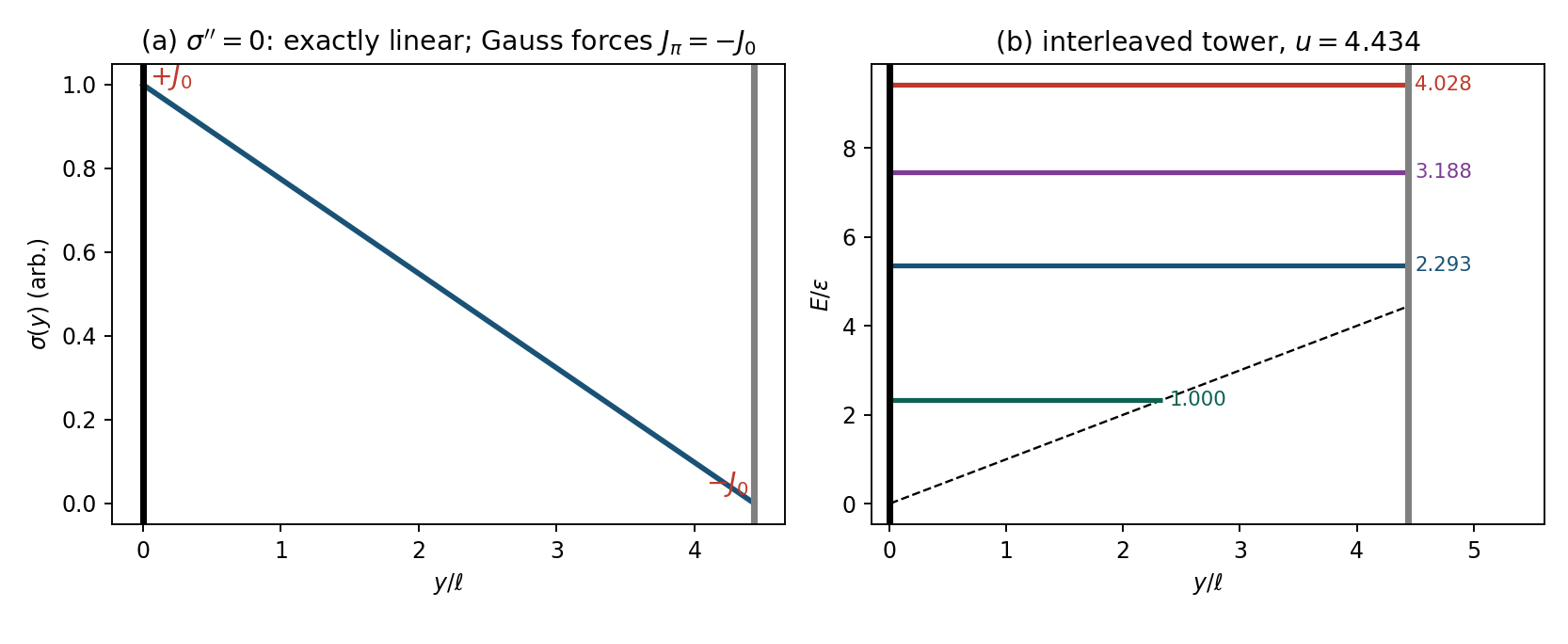
\includegraphics[width=0.98\textwidth]{fig1_welltower.png}
\caption{(a) The brane-sourced profile: Laplace's equation makes it exactly linear between the boundaries; the fold at each boundary is the tadpole, and Gauss's law forces the charges opposite. (b) The interleaved tower on the derived well at $u=\pi R/\ell=4.43$: even branch (Neumann at the sourced wall) and odd branch (Dirichlet) alternate, giving $1:2.293:3.188:4.028$ with nothing adjusted; the fourth level's turning point approaches the far wall --- it is the level that measures $u$. [\texttt{u\_derive.py}, \texttt{figures2.py}]}
\label{fig:welltower}
\end{figure}

\section{The interleaved tower, and the triplet that closes}
\subsection{The spectrum}
On the linear well the mode equation is the Airy problem of the quantum bouncer, one dimension up from the ultracold-neutron states quoted in Article I. The boundary conditions interleave two branches: the even branch, Neumann at the sourced wall ($\psi'(0)=0$ --- maximal, not vanishing, at our brane), and the odd branch, Dirichlet ($\psi(0)=0$); both terminate on the far wall at $y=\pi R$. Solving with nothing adjusted returns the tower
\begin{equation}
E_{1}:E_{2}:E_{3}:E_{4}\;=\;1:2.29:3.19:4.03\;\;(2.294,\,3.189,\,4.029\ \text{at the dossier's grid}),
\end{equation}
pure numbers of the geometry, independent of every open input. The characteristic length and energy are $\ell=(\hslash^{2}/2m_{\Phi}F)^{1/3}=5.81~\mu$m and $\varepsilon=F\ell=24$~meV. In physical units the four bound levels sit at $24$, $55$, $77$ and $96$~meV above the well floor --- the entire discrete sector of the framework spans a factor four in energy, all of it inside the decade that Article IV's shadow relation predicts and none of it adjustable. [Derived]

\subsection{$u$ is an output}
The interval-to-well ratio $u\equiv\pi R/\ell$ was, in earlier statements, read off the spectrum. It is in fact computable: with $R$ fixed by Article I's calibration, $F$ by the tower scale, and $m_{\Phi}$ by the framework's single meV input, one finds
\begin{equation}
u=\frac{\pi R}{\ell}=4.43 ,
\end{equation}
in agreement with the value the interleaved fit requires --- the triplet $(\ell,\varepsilon,u)$ closes on \emph{one} scale,
\begin{equation}
m_{\Phi}=\varepsilon\approx 1/R=24~\mathrm{meV},
\label{eq:knot}
\end{equation}
and what once looked like several coincidences of the meV sector is one: Eq.~(\ref{eq:knot}) is the knot, and Article IV explains it as the gravitational shadow of the TeV wall. Because the fourth ratio also \emph{measures} $u$ (\S4), the quantity is both derived and observable: a closed test. [Derived]

\section{The two dials}
\subsection{The mass of the source}
A massive source bends the profile: $\sigma''=m_{\sigma}^{2}\sigma$ turns the line into a $\sinh$, deforming the well by $(m_{\sigma}\pi R)^{2}/6$ at the far edge. Propagated through the spectrum, the tower \emph{ratios} --- the observable --- shift about five times less than the profile does, and the numerical dial reads:
\begin{equation}
\text{ratios measured at }1\%\quad\Longrightarrow\quad m_{\sigma}<4.3~\mathrm{meV}.
\end{equation}
If the dark tower is ever spectroscopically resolved, it measures the mass of the field that shapes its own well. [Derived]
\subsection{The fourth ratio}
The first three levels have turning points well inside the corridor; the fourth is the only one whose turning point approaches the far wall, and its ratio is correspondingly the only one sensitive to $u$ --- shifting measurably as $u$ varies around $4.43$. The tower thus carries two independent dials: levels one to three read $m_{\sigma}$, level four reads the geometry. [Derived]

\begin{figure}[t]
\centering
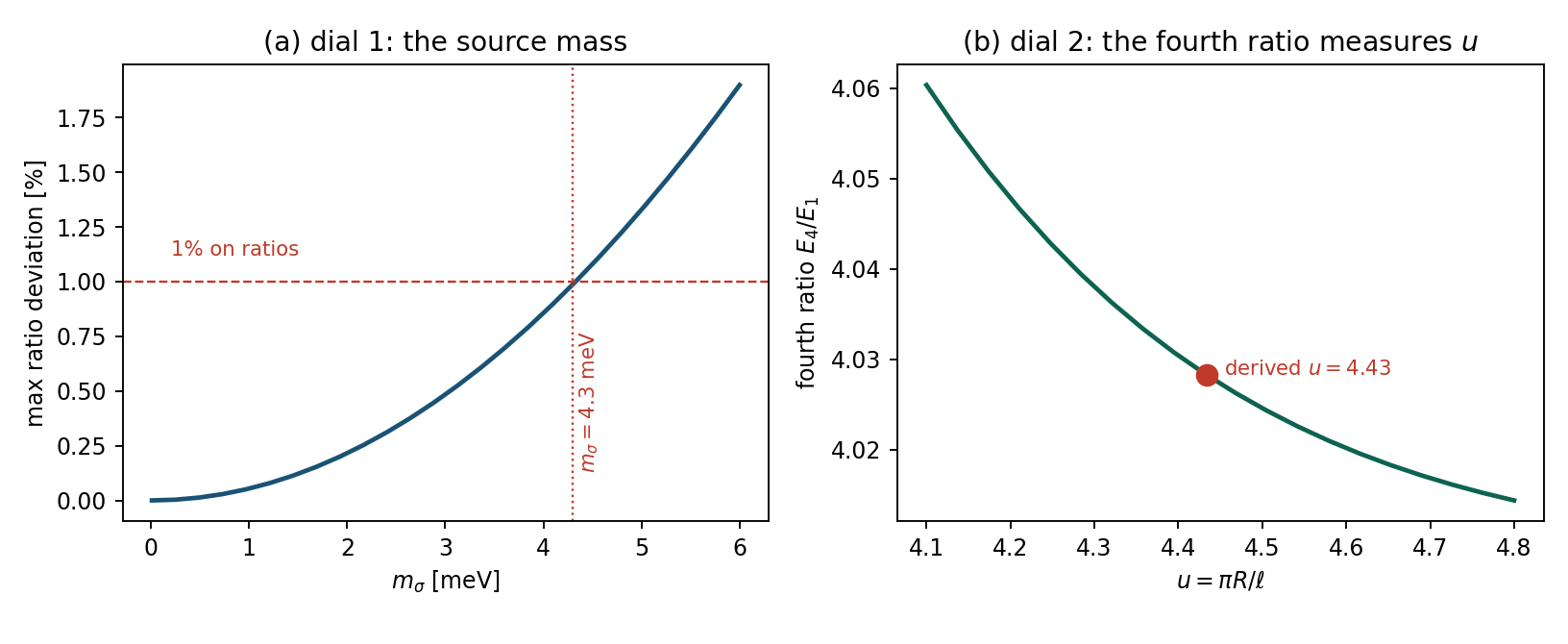
\includegraphics[width=0.9\textwidth]{fig2_dials.png}
\caption{The two dials. Left: maximal tower-ratio deviation versus the source mass $m_{\sigma}$; the $1\%$ line crosses at $4.3$~meV. Right: the fourth ratio versus the interval parameter $u$; the derived value $u=4.43$ (marker) sits where the interleaved tower requires it. [\texttt{J1J2\_capaciteur.py}, \texttt{u\_derive.py}]}
\label{fig:dials}
\end{figure}

\section{The amplitude accounting, closed}
Article I wrote the covariant vertex and its reduction, $\alpha_{b}=c_{b}\sqrt{2w_{1}}$, with the boundary weight $w_{1}\equiv\pi R\,|\psi_{1}(0)|^{2}$ left to be computed here. On the derived well the ground state is the \emph{even} branch --- maximal at the sourced wall --- and its normalised boundary weight is
\begin{equation}
w_{1}=u\,|\hat{\psi}_{1}(0)|^{2}=5.5\qquad\Longrightarrow\qquad \alpha_{b}=3.3\,c_{b}.
\end{equation}
The framework's requirement analysis lists the galactic response amplitudes demanded by the phenomenology of Article III; the closed accounting translates them into the ultraviolet vertex:
\begin{center}\small
\begin{tabular}{lcccc}
\toprule
required $\alpha_{b}$ & 1.0 & 2.0 & 10 & 512\\
required $c_{b}$ & 0.30 & 0.61 & 3.0 & 155\\
\bottomrule
\end{tabular}
\end{center}
The benchmark responses sit at $c_{b}=0.30$--$0.61$: order unity, with nothing forced --- the naturalness statement of the series, now with its number. [The companion's tree-level bound, $c_{b}\leq\sqrt{255/56}=2.13$, excludes the two large entries of the table, $c_{b}=3.0$ and $c_{b}=155$, leaving exactly the low branch that the galactic accounting independently preferred. The value of $c_{b}$ is not thereby derived and its label is unchanged. See Appendix~C.] A historical remark belongs in one sentence: an early accounting of this framework carried an apparent deficit of $4.5\times10^{7}$ in the brane coupling, which dissolved when the bulk normalisation and the boundary weight were joined in the single identity above --- the deficit was the trace of two normalisations never joined, and the closed form is the repair. One counting subtlety, inherited from the framework's amplitude analysis, deserves its place here because referees will look for it. The \emph{galactic} response of Article III proceeds through a single boundary vertex --- the medium is sourced once, coherently --- so it scales as $\alpha_{b}\propto c_{b}\sqrt{2w_{1}}$; a \emph{laboratory} force mediated by the tower would require two vertices and scale as $\alpha_{b}^{2}\propto c_{b}^{2}\,(2w_{1})$, which is one reason the short-range map of Article I stays clean even before the parity and charge arguments of \S6: the double-vertex channel is doubly suppressed, and the single-vertex channel has no laboratory realisation --- it needs a medium to push on, and the solar bubble of Article III contains none. The two powers of $w_{1}$ are not interchangeable, and an early accounting that mixed them is part of the historical note above. [Derived; $c_{b}$ remains Input-natural, per Article I]

\section{What the source field does not do}
\emph{No fifth force.} The tadpole couples $\sigma$ to the unit operator of the brane --- a tension term --- not to the matter density: an atom carries no $\sigma$ charge, the tree-level Yukawa between test masses vanishes, and the short-range landscape of Article I is unchanged --- the exclusion map stays clean. Induced channels are computed and negligible: $\sigma$--radion mixing is $\theta\sim V_{\sigma}/V_{\rm stab}\approx2\times10^{-57}$, a force ratio to gravity below $10^{-113}$; the halo background $g\langle\Phi^{2}\rangle$ sources $\sigma$ only between dark concentrations. [Derived]

\emph{No stabilisation.} The radion is a metric mode with Planckian inertia, $m_{r}\sim\sqrt{V_{\rm stab}}/\MPl$; the capacitor lives at the meV scale, and its contribution to the radion mass is $\sim4\times10^{-31}$~eV --- twenty-eight orders below the framework's window. The same field \emph{can} be promoted to a Goldberger--Wise stabiliser by TeV-scale boundary values \cite{GW99}, but then the well slope and the stabilisation energy decouple through the free coupling: the hoped-for structural link between them is refuted, and the honest structure is \textbf{two independent origins} --- a TeV core (tension, stabilisation, thickness) and a meV source sector (the well). Article IV explains why the two nonetheless speak to each other. [Derived no-go]

\emph{One declared tension, and the framework's most severe.} The background energy of the capacitor must fit inside the dark-energy budget, $\rho_{\sigma}=(\pi R/8)J_{0}^{2}\leq\rho_{\Lambda}$, which caps $J_{0}\leq4\times10^{-29}~\mathrm{GeV}^{5/2}$ and, with $F$ fixed, requires $g\gtrsim4\times10^{7}~\mathrm{GeV}^{1/2}\simeq2\times10^{3}\sqrt{\Mfive}$ --- a coupling three orders above its natural size, or a partial cancellation of the background energy. This is the framework's most severe naturalness tension, and it must be stated plainly: the well that the framework derives so cleanly demands, at its source, a coupling that the framework cannot justify. The tension is not hidden, not minimised, not explained away: it is declared, and it is filed in the class where it belongs --- the cosmological-constant problem, inherited from the residual $\Lambda$ of Article I \S2, met here from a second direction. The framework does not resolve this tension; it locates it.

The interrogation must be recorded, because it is what licenses the label. Two natural protections were tested, and both failed. First, 't~Hooft technical naturalness: does $J_{0}\to0$ restore a symmetry? The shift symmetry $\sigma\to\sigma+c$ is restored in the limit $J_{0}\to0$, $m_{\sigma}\to0$, but the $\Phi$ loop regenerates a tadpole fifty-one orders too large at the fundamental cutoff $\Mfive$ --- the symmetry is not protected against the very sector that generates the well. Second, TeV-scale supersymmetry: does the superpartner cancel the loop? At the supersymmetric cutoff $M_{S}\simeq7.6$~TeV the loop remains forty-one orders too large; protecting a meV tadpole would require supersymmetry unbroken down to the meV scale, which nothing in this framework provides. The tension is therefore definitively of the cosmological-constant class --- not a technical-naturalness problem that a symmetry could solve, but a vacuum-energy problem that inherits the deepest open question of the series. [Interrogation: recorded; verdict: S-3] Alongside it, the initial occupation fractions of the tower are a choice: no sum identity or hidden symmetry of the Airy zeros fixes them, a negative result established by the framework's own derivation programme; the flat-profile fractions used in Article III are [Posited] and labelled so. [Open, declared / S-3]

\section{How this article dies}
(i) \emph{Anharmonicity of the wrong shape:} the two roads both predict deviations of the $\sinh$ family; a measured tower anharmonicity not of that form kills the derived well outright. (ii) \emph{Ratios without a home:} joint level ratios inconsistent with any pair $(m_{\sigma},u)$ falsify the construction --- two dials, no third knob. (iii) \emph{A force at the source's range:} any laboratory Yukawa attributable to $\sigma$ contradicts the minimal coupling structure, which forbids one. (iv) \emph{The tension road:} if the wall scale is ever pinned outside $2$--$13$~TeV, the gravitational slope fails, removing half of \S2 and the tension window with it. Article III now sets this tower in motion: the reservoir, the condensate, the drip, and the one response the universe actually shows us.


% ═══════════════════════════════════════════════════════════════════════════
%  APPENDICE DE LIAISON — identique dans les sept articles.
%  % ═══════════════════════════════════════════════════════════════════════════
%  APPENDICE DE LIAISON — identique dans les sept articles.
%  % ═══════════════════════════════════════════════════════════════════════════
%  APPENDICE DE LIAISON — identique dans les sept articles.
%  \input{appendix-where} juste avant \begin{thebibliography} ou la biblio.
%  Il répond à : qui vit où, et qu'est-ce que la série a changé en cours de route.
% ═══════════════════════════════════════════════════════════════════════════
\section*{Appendix: which sector lives where, and what changed}
\addcontentsline{toc}{section}{Appendix: which sector lives where}

The series was written over several months and \textbf{two of its assignments moved}.
A reader who meets the articles out of order is owed an explicit map rather than an
inference, so it is given here, identically in all seven papers.

\subsection*{A.1 The three locations}
The geometry has three places where physics can sit: the \emph{brane} at $y=0$,
the \emph{bulk} of the $8.2\,\mu$m interval, and the \emph{far wall} at $y=\pi R$.
\begin{center}\small
\begin{tabular}{llll}\toprule
sector & lives on & carried by & established in\\\midrule
ordinary matter & \textbf{brane} & thin core, Standard Model & I\\
gravity, radion, graviton & \textbf{bulk} & five-dimensional fields & I\\
the mediator $\Phi$ and its tower & \textbf{bulk} & Airy states of the $|y|$ well & II\\
the galactic response & \textbf{bulk} $\to$ brane & $\Phi$ exchange between baryons & III\\
dark matter & \textbf{see A.2} & --- & III, revisited in VI\\
dark energy & \textbf{see A.3} & --- & III, revisited in VI\\
hidden gauge sector & \textbf{far wall} & eight D8 and one O8 & V\\\bottomrule
\end{tabular}
\end{center}

\subsection*{A.2 Dark matter: the reservoir, and what the wall reading adds}
Articles~I--IV place dark matter in the \emph{bulk}: the excited states of the Airy
tower, populated cold at birth, collisionless, carrying at least $98.6\%$ of the dark
sector's density. That assignment does the work in three places. It makes structure
formation identical to cold dark matter at linear order. It answers the Bullet Cluster
by mass budget alone --- cluster masses are cluster masses, and the lensing tracks the
reservoir, which is why the lensing--dynamics difficulty of purely modified dynamics is
not inherited. And it fixes the radiation budget of Article~I.

Article~VI proposes a different reading: dark matter as the ordinary matter of the six
other regions of the same wall, seen through the bulk, giving
$\Omega_{\rm DM}/\Omega_b=N_{\rm regions}-1=6$ against an observed $5.31$.
\textbf{These are not the same statement, and we do not pretend otherwise.}

What they share is everything the phenomenology uses: in both readings the dark
component is cold, collisionless, and carries the mass, so lensing, the Bullet Cluster
and linear structure formation are unaffected. What differs is the \emph{constituent}:
quanta of $\Phi$ in the first, baryons of other regions in the second.
\textbf{The two are compatible if the tower reservoir is not required to be the whole
of the dark matter} --- and Article~III's own argument only requires it to dominate the
budget, not to be exhaustive. \Open

\subsection*{A.3 Dark energy: a bulk scalar, then a brane curvature}
Articles~I--IV treat $\Phi$ as the dark-energy candidate --- a bulk scalar engine. That
attempt \emph{failed by forty orders of magnitude}: a four-dimensional scalar cannot
reach $2.4$~meV from a $10^{-13}$~eV engine scale. The failure is recorded, not hidden.

Article~VI relocates dark energy \emph{to the brane}, as the extrinsic curvature of the
D8 wall in the cosmological bulk, $\Lambda_4=\varepsilon^2(1/R)^4$ with
$\varepsilon\simeq10^{-2}$. The mechanism supplies $(1/R)^4$ outright and leaves a gap
of $10^4$ rather than $10^{40}$. \textbf{$\Phi$ is correspondingly demoted from
dark-energy candidate to dark-sector mediator}, which is the role Articles~II and III
already gave it in every equation they actually use. \Candidate, declared tuning.

\subsection*{A.4 The radial acceleration relation, and what makes galaxies turn}
The relation is the one place where brane and bulk are \emph{both} indispensable, and
where nothing has moved since Article~III.

Baryons sit on the brane. They source $\Phi$, which propagates in the bulk with mass
$m_\Phi=24$~meV and hence Compton range $8.2\,\mu$m --- microscopic, so no fifth force
acts between laboratory bodies. What acts at galactic scale is not the free field but
the \emph{medium}: the coherent component of the dark sector responds to the baryonic
distribution, and that response, read back on the brane, is the extra acceleration.
The response saturates, which is why it produces a relation --- an acceleration scale
$g_\dagger$ --- rather than a rescaling of Newton's constant.

Three consequences, all in Article~III and unchanged:
\begin{itemize}\itemsep2pt
\item the response couples to the trace $T^\mu_{\ \mu}$, hence to mass and not to
      composition; the universality is bounded on 171 SPARC galaxies;
\item the response is carried by at most $1.4\%$ of the dark sector, the coherent part,
      so it never competes with the reservoir in the mass budget --- \textbf{galaxies
      turn because of the medium, they weigh because of the reservoir};
\item the response \emph{dies} in weak field, which is the ultra-diffuse galaxy test,
      and it dies in a decoherence bubble around the Sun, which is why Cassini is
      satisfied identically rather than by tuning.
\end{itemize}
\textbf{Neither relocation of A.2 or A.3 touches this.} The galactic response was never
assigned to the dark-energy sector, and it is not the reservoir either; it is the third
role, and it is the one the framework was built to explain.

\subsection*{A.5 What a reader should carry between articles}
Articles~I--IV stand on their own evidence and are not modified by V--VII: no result of
theirs is derived from the string embedding, and the embedding cannot promote any of
their labels. What V--VII add is an ultraviolet origin for one constant, a candidate
geometry, and two consequences of that geometry. What they \emph{change} is recorded
above and nowhere else: two relocations, both declared, neither retroactive.
 juste avant \begin{thebibliography} ou la biblio.
%  Il répond à : qui vit où, et qu'est-ce que la série a changé en cours de route.
% ═══════════════════════════════════════════════════════════════════════════
\section*{Appendix: which sector lives where, and what changed}
\addcontentsline{toc}{section}{Appendix: which sector lives where}

The series was written over several months and \textbf{two of its assignments moved}.
A reader who meets the articles out of order is owed an explicit map rather than an
inference, so it is given here, identically in all seven papers.

\subsection*{A.1 The three locations}
The geometry has three places where physics can sit: the \emph{brane} at $y=0$,
the \emph{bulk} of the $8.2\,\mu$m interval, and the \emph{far wall} at $y=\pi R$.
\begin{center}\small
\begin{tabular}{llll}\toprule
sector & lives on & carried by & established in\\\midrule
ordinary matter & \textbf{brane} & thin core, Standard Model & I\\
gravity, radion, graviton & \textbf{bulk} & five-dimensional fields & I\\
the mediator $\Phi$ and its tower & \textbf{bulk} & Airy states of the $|y|$ well & II\\
the galactic response & \textbf{bulk} $\to$ brane & $\Phi$ exchange between baryons & III\\
dark matter & \textbf{see A.2} & --- & III, revisited in VI\\
dark energy & \textbf{see A.3} & --- & III, revisited in VI\\
hidden gauge sector & \textbf{far wall} & eight D8 and one O8 & V\\\bottomrule
\end{tabular}
\end{center}

\subsection*{A.2 Dark matter: the reservoir, and what the wall reading adds}
Articles~I--IV place dark matter in the \emph{bulk}: the excited states of the Airy
tower, populated cold at birth, collisionless, carrying at least $98.6\%$ of the dark
sector's density. That assignment does the work in three places. It makes structure
formation identical to cold dark matter at linear order. It answers the Bullet Cluster
by mass budget alone --- cluster masses are cluster masses, and the lensing tracks the
reservoir, which is why the lensing--dynamics difficulty of purely modified dynamics is
not inherited. And it fixes the radiation budget of Article~I.

Article~VI proposes a different reading: dark matter as the ordinary matter of the six
other regions of the same wall, seen through the bulk, giving
$\Omega_{\rm DM}/\Omega_b=N_{\rm regions}-1=6$ against an observed $5.31$.
\textbf{These are not the same statement, and we do not pretend otherwise.}

What they share is everything the phenomenology uses: in both readings the dark
component is cold, collisionless, and carries the mass, so lensing, the Bullet Cluster
and linear structure formation are unaffected. What differs is the \emph{constituent}:
quanta of $\Phi$ in the first, baryons of other regions in the second.
\textbf{The two are compatible if the tower reservoir is not required to be the whole
of the dark matter} --- and Article~III's own argument only requires it to dominate the
budget, not to be exhaustive. \Open

\subsection*{A.3 Dark energy: a bulk scalar, then a brane curvature}
Articles~I--IV treat $\Phi$ as the dark-energy candidate --- a bulk scalar engine. That
attempt \emph{failed by forty orders of magnitude}: a four-dimensional scalar cannot
reach $2.4$~meV from a $10^{-13}$~eV engine scale. The failure is recorded, not hidden.

Article~VI relocates dark energy \emph{to the brane}, as the extrinsic curvature of the
D8 wall in the cosmological bulk, $\Lambda_4=\varepsilon^2(1/R)^4$ with
$\varepsilon\simeq10^{-2}$. The mechanism supplies $(1/R)^4$ outright and leaves a gap
of $10^4$ rather than $10^{40}$. \textbf{$\Phi$ is correspondingly demoted from
dark-energy candidate to dark-sector mediator}, which is the role Articles~II and III
already gave it in every equation they actually use. \Candidate, declared tuning.

\subsection*{A.4 The radial acceleration relation, and what makes galaxies turn}
The relation is the one place where brane and bulk are \emph{both} indispensable, and
where nothing has moved since Article~III.

Baryons sit on the brane. They source $\Phi$, which propagates in the bulk with mass
$m_\Phi=24$~meV and hence Compton range $8.2\,\mu$m --- microscopic, so no fifth force
acts between laboratory bodies. What acts at galactic scale is not the free field but
the \emph{medium}: the coherent component of the dark sector responds to the baryonic
distribution, and that response, read back on the brane, is the extra acceleration.
The response saturates, which is why it produces a relation --- an acceleration scale
$g_\dagger$ --- rather than a rescaling of Newton's constant.

Three consequences, all in Article~III and unchanged:
\begin{itemize}\itemsep2pt
\item the response couples to the trace $T^\mu_{\ \mu}$, hence to mass and not to
      composition; the universality is bounded on 171 SPARC galaxies;
\item the response is carried by at most $1.4\%$ of the dark sector, the coherent part,
      so it never competes with the reservoir in the mass budget --- \textbf{galaxies
      turn because of the medium, they weigh because of the reservoir};
\item the response \emph{dies} in weak field, which is the ultra-diffuse galaxy test,
      and it dies in a decoherence bubble around the Sun, which is why Cassini is
      satisfied identically rather than by tuning.
\end{itemize}
\textbf{Neither relocation of A.2 or A.3 touches this.} The galactic response was never
assigned to the dark-energy sector, and it is not the reservoir either; it is the third
role, and it is the one the framework was built to explain.

\subsection*{A.5 What a reader should carry between articles}
Articles~I--IV stand on their own evidence and are not modified by V--VII: no result of
theirs is derived from the string embedding, and the embedding cannot promote any of
their labels. What V--VII add is an ultraviolet origin for one constant, a candidate
geometry, and two consequences of that geometry. What they \emph{change} is recorded
above and nowhere else: two relocations, both declared, neither retroactive.
 juste avant \begin{thebibliography} ou la biblio.
%  Il répond à : qui vit où, et qu'est-ce que la série a changé en cours de route.
% ═══════════════════════════════════════════════════════════════════════════
\section*{Appendix: which sector lives where, and what changed}
\addcontentsline{toc}{section}{Appendix: which sector lives where}

The series was written over several months and \textbf{two of its assignments moved}.
A reader who meets the articles out of order is owed an explicit map rather than an
inference, so it is given here, identically in all seven papers.

\subsection*{A.1 The three locations}
The geometry has three places where physics can sit: the \emph{brane} at $y=0$,
the \emph{bulk} of the $8.2\,\mu$m interval, and the \emph{far wall} at $y=\pi R$.
\begin{center}\small
\begin{tabular}{llll}\toprule
sector & lives on & carried by & established in\\\midrule
ordinary matter & \textbf{brane} & thin core, Standard Model & I\\
gravity, radion, graviton & \textbf{bulk} & five-dimensional fields & I\\
the mediator $\Phi$ and its tower & \textbf{bulk} & Airy states of the $|y|$ well & II\\
the galactic response & \textbf{bulk} $\to$ brane & $\Phi$ exchange between baryons & III\\
dark matter & \textbf{see A.2} & --- & III, revisited in VI\\
dark energy & \textbf{see A.3} & --- & III, revisited in VI\\
hidden gauge sector & \textbf{far wall} & eight D8 and one O8 & V\\\bottomrule
\end{tabular}
\end{center}

\subsection*{A.2 Dark matter: the reservoir, and what the wall reading adds}
Articles~I--IV place dark matter in the \emph{bulk}: the excited states of the Airy
tower, populated cold at birth, collisionless, carrying at least $98.6\%$ of the dark
sector's density. That assignment does the work in three places. It makes structure
formation identical to cold dark matter at linear order. It answers the Bullet Cluster
by mass budget alone --- cluster masses are cluster masses, and the lensing tracks the
reservoir, which is why the lensing--dynamics difficulty of purely modified dynamics is
not inherited. And it fixes the radiation budget of Article~I.

Article~VI proposes a different reading: dark matter as the ordinary matter of the six
other regions of the same wall, seen through the bulk, giving
$\Omega_{\rm DM}/\Omega_b=N_{\rm regions}-1=6$ against an observed $5.31$.
\textbf{These are not the same statement, and we do not pretend otherwise.}

What they share is everything the phenomenology uses: in both readings the dark
component is cold, collisionless, and carries the mass, so lensing, the Bullet Cluster
and linear structure formation are unaffected. What differs is the \emph{constituent}:
quanta of $\Phi$ in the first, baryons of other regions in the second.
\textbf{The two are compatible if the tower reservoir is not required to be the whole
of the dark matter} --- and Article~III's own argument only requires it to dominate the
budget, not to be exhaustive. \Open

\subsection*{A.3 Dark energy: a bulk scalar, then a brane curvature}
Articles~I--IV treat $\Phi$ as the dark-energy candidate --- a bulk scalar engine. That
attempt \emph{failed by forty orders of magnitude}: a four-dimensional scalar cannot
reach $2.4$~meV from a $10^{-13}$~eV engine scale. The failure is recorded, not hidden.

Article~VI relocates dark energy \emph{to the brane}, as the extrinsic curvature of the
D8 wall in the cosmological bulk, $\Lambda_4=\varepsilon^2(1/R)^4$ with
$\varepsilon\simeq10^{-2}$. The mechanism supplies $(1/R)^4$ outright and leaves a gap
of $10^4$ rather than $10^{40}$. \textbf{$\Phi$ is correspondingly demoted from
dark-energy candidate to dark-sector mediator}, which is the role Articles~II and III
already gave it in every equation they actually use. \Candidate, declared tuning.

\subsection*{A.4 The radial acceleration relation, and what makes galaxies turn}
The relation is the one place where brane and bulk are \emph{both} indispensable, and
where nothing has moved since Article~III.

Baryons sit on the brane. They source $\Phi$, which propagates in the bulk with mass
$m_\Phi=24$~meV and hence Compton range $8.2\,\mu$m --- microscopic, so no fifth force
acts between laboratory bodies. What acts at galactic scale is not the free field but
the \emph{medium}: the coherent component of the dark sector responds to the baryonic
distribution, and that response, read back on the brane, is the extra acceleration.
The response saturates, which is why it produces a relation --- an acceleration scale
$g_\dagger$ --- rather than a rescaling of Newton's constant.

Three consequences, all in Article~III and unchanged:
\begin{itemize}\itemsep2pt
\item the response couples to the trace $T^\mu_{\ \mu}$, hence to mass and not to
      composition; the universality is bounded on 171 SPARC galaxies;
\item the response is carried by at most $1.4\%$ of the dark sector, the coherent part,
      so it never competes with the reservoir in the mass budget --- \textbf{galaxies
      turn because of the medium, they weigh because of the reservoir};
\item the response \emph{dies} in weak field, which is the ultra-diffuse galaxy test,
      and it dies in a decoherence bubble around the Sun, which is why Cassini is
      satisfied identically rather than by tuning.
\end{itemize}
\textbf{Neither relocation of A.2 or A.3 touches this.} The galactic response was never
assigned to the dark-energy sector, and it is not the reservoir either; it is the third
role, and it is the one the framework was built to explain.

\subsection*{A.5 What a reader should carry between articles}
Articles~I--IV stand on their own evidence and are not modified by V--VII: no result of
theirs is derived from the string embedding, and the embedding cannot promote any of
their labels. What V--VII add is an ultraviolet origin for one constant, a candidate
geometry, and two consequences of that geometry. What they \emph{change} is recorded
above and nowhere else: two relocations, both declared, neither retroactive.

\toolsstatement
\traceability{2}{The Airy tower, the boundary weight $w_1$ and the coupling table are produced by \texttt{scripts/tower.py}.}
\bibliographystyle{unsrt}\bibliography{ddf-refs}
\appendix
\section{The EXP-B expedition}
The results presented here were obtained through the EXP-B expedition (v1.0 + v1.1 + audit), a systematic exploration of whether a minimal 5D field model can derive the TeV scales of the framework from a single origin.

\textbf{Phase 1 (v1.0).} The initial thesis was that the minimal wall-soliton $\sigma(y)=v\tanh(y/\delta)$ is the natural candidate for the structural link between the three TeV scales. This was refuted by pre-registered criterion M3: a kink of $174~\mu$m cannot fit inside a corridor of $\pi R=25.8~\mu$m --- the ``wall'' would be $7\times$ wider than the dimension itself. On the interval, $\tanh(y/\delta)$ with $\delta\gg\pi R$ is not a wall but a pure gradient, $\sigma=vy/\delta+\mathcal{O}((y/\delta)^{3})$.

\textbf{Phase 2 (corrections C1--C6).} The correct minimal object is the capacitor: a field $\sigma$ sourced on both branes obeys $\sigma''=0$ in the 5D vacuum, giving an exactly linear profile with zero shape parameters. This is the construction of \S2.2 of the main text.

\textbf{Phase 3 (v1.1).} The capacitor was formalised ($\sigma$ $\mathbb{Z}_2$-even; Gauss's law forces $J_{0}+J_{\pi}=0$), the spectrum computed, and the two dials identified ($m_\sigma<4.3$~meV; the fourth ratio measures $u$).

\textbf{Phase 4 (audit).} The hoped-for structural link ($V_{\rm stab}\leftrightarrow k$) via Goldberger--Wise was refuted. The radion carries Planckian inertia, and the capacitor lives at the meV scale: its contribution to the radion mass is $\sim4\times10^{-31}$~eV, twenty-eight orders below the required 9~meV. The two sectors are genuinely independent; the hoped-for bonus dies honestly.

\textbf{Phase 5 (G6).} The Yukawa amplitude of $\sigma$ was computed and found invisible (tree-level force between test masses zero; induced channels $<10^{-100}\times$ gravity). The range spectrum of the framework is unchanged.

The expedition produced one positive result --- the linear well derived from brane sources --- and several honest no-go results (the wall-soliton minimal is dead; the structural link $V_{\rm stab}\leftrightarrow k$ is refuted; the Yukawa is invisible). This is the standard of the series: results are stated with their shadows declared, not hidden.

\section{Detailed results of the EXP-B expedition}
\begin{center}\small
\textbf{Acquired}\\[2pt]
\begin{tabular}{llll}\toprule
\# & Result & Status & Source\\\midrule
R1 & The capacitor $\sigma$ $\mathbb{Z}_2$-even produces the linear well $k$ & [Derived] & J1$'$\\
R2 & Gauss's law $J_{0}+J_{\pi}=0$ forced & [Derived] & J1$'$, G3\\
R3 & T1 in prediction mode (interleaved-tower ratios at $m_\sigma=0$; the fourth measures $u$) & [Derived] & J2$'$\\
R4 & The dial $m_\sigma<4.3$ meV (on the ratios) & [Confirmed] & J2$'$, A1\\
R5 & C4: $\sqrt{k}=29$ meV $\approx\varepsilon=24$ meV & [Confirmed] & J2$'$\\
R6 & T4b: two origins (TeV + meV), independent & [Confirmed] & J4$'$, A3\\
R7 & T0: interleaved tower = target convention & [Derived] & J1\\
R8 & Yukawa of $\sigma$ invisible (G6) & [Derived] & G6\\\bottomrule
\end{tabular}\\[8pt]
\textbf{Refuted}\\[2pt]
\begin{tabular}{llll}\toprule
\# & Result & Status & Source\\\midrule
F1 & Link ($V_{\rm stab}\leftrightarrow k$) as structural link & [Refuted] & A2, A3\\
F2 & ``Tension dial vs radion window'' & [Artefact] & A2\\
F3 & The $\sigma$ $\mathbb{Z}_2$-odd for this job & [Dead] & G1\\
F4 & The minimal wall-soliton $\tanh$ & [Dead] & C2\\
F5 & The v1.0 thesis (one $\tanh$ for two jobs) & [Refuted] & C2\\\bottomrule
\end{tabular}\\[8pt]
\textbf{Open / Parked}\\[2pt]
\begin{tabular}{llll}\toprule
\# & Result & Status & Source\\\midrule
O1 & Precise value of $c_{b}$ (table $0.30/0.61/3.0/155$; the two large entries are excluded by the companion, Appendix~C) & Step 2 & J3$'$\\
O2 & Three TeV scales at the thin core (T4a) & Step 2, parked & J4$'$\\
O3 & Naturalness tension $\sim\mathcal{O}(10^{3})$ (G6) & Declared & G6\\
P1 & Step 2 (SUSY microphysics of the core) & Declared future work & A4\\\bottomrule
\end{tabular}
\end{center}


\section*{Appendix C: what the companion does, and does not, provide}
\addcontentsline{toc}{section}{Appendix C}
\label{app:companion}

A fifth article --- \emph{The Dark Dimension Framework from Type~I$'$ strings}, cited here as the companion --- asks whether the geometry of Articles~I--IV admits an ultraviolet completion. It is deposited together with this series so that a reader who asks \emph{where does this constant come from?} has somewhere to look. Three statements govern how it may be used.

\paragraph{It is a companion, not a foundation.} Every result, label and executioner of Articles~I--IV is established at the effective-theory level and stands or falls on its own evidence. If the companion's embedding is refuted tomorrow, nothing in this article changes. The converse also holds: the companion cannot promote a label here, and none of its findings has been used to do so.

\paragraph{What it establishes.} The companion shows that the framework's boundary conditions ($J_{0}+J_{\pi}=0$) are literally the Ramond--Ramond tadpole cancellation of a Type~I$'$ orientifold; it derives, at tree level, the coupling vector through which brane tension reaches the bulk scalar, obtaining three integer norm identities and an upper bound on the boundary constant, $c_{b}\leq\sqrt{255/56}=2.13$; it establishes two autonomous negative results (five independent moduli-pinning mechanisms fail, and massive type~IIA is incompatible with a mesoscopic interval); and it exhibits one explicit candidate vacuum that passes every computable test. For the present article the relevant item is the coupling table of \S5: the companion's bound $c_{b}\leq2.13$ excludes the two large benchmarks, $c_{b}=3.0$ and $c_{b}=155$, leaving the low branch that the galactic accounting independently preferred. Two further checks were run against this article and passed: the boundary weight $w_{1}=5.5$ is confirmed, and the tower ratios are reproduced by the well on the covering space with both parities retained.

\paragraph{What it does not establish.} It does not derive the value of $c_{b}$. That value depends on the mixing angle of the light modulus, which in turn depends on string-loop coefficients that are not computable for a general Calabi--Yau manifold --- a frontier of that field, not of this construction. The companion therefore closes with a conditional statement, not a number. \textbf{Accordingly, no label in Articles~I--IV is altered by it}: what was [Input, natural] remains so, and what was [Open, declared] remains open. A further consequence is recorded here rather than in the body: the companion's flat subspace is two-dimensional, so the moduli sector carries \emph{two} light scalars rather than one. Their towers differ by four parts in $10^{8}$, so the amplitude accounting of this article is unaffected --- no experiment separates them --- and what a fifth-force measurement returns is the sum of the squared couplings. That sum is fixed by the companion's geometry without any string-loop coefficient.

\end{document}